As described in Section~\ref{sec:physics-lbnosc-senscalc}, the effect of systematic uncertainty on
experimental sensitivity is approximated by allowing the neutrino oscillation
parameters to vary within the uncertainty in the global fit to neutrino data
\cite{Gonzalez-Garcia:2014bfa} and by allowing the  signal and background rates
to vary based on normalization uncertainties. In the sensitivities presented there, the
signal normalization uncertainties are 5\% on the \numu and \anumu samples and
2\% on the \nue and \anue samples. These four signal normalization uncertainties
are treated as 100\% uncorrelated so that the 2\% normalization uncertainty on the
\nue sample represents a residual normalization uncertainty after constraints
from the near detector, the \numu disappearance samples, and the \anue sample have been applied.
The normalization uncertainties on background to these samples and the correlation among these
uncertainties are presented in Table~\ref{tab:bgnormsys}. The result of the correlations
presented in Table~\ref{tab:bgnormsys} is that there are five independent background
normalization uncertainties: beam \nue, beam \anue, \numu/NC background to appearance mode,
NC background to disappearance mode, and $\nu_\tau$.

\begin{table}[!tb]
  \begin{center}
    \caption{Normalization uncertainties and correlations for background to the \nue, \anue, \numu, and \anumu data samples.}
    \label{tab:bgnormsys}
    \begin{tabular}{l|c|l} \hline\hline
      Background & Normalization Uncertainty & Correlations \\ \hline
      \multicolumn{3}{l}{For \nue/\anue appearance:} \\ 
      Beam \nue & 5\% & Uncorrelated in \nue and \anue samples \\
      NC      & 5\%  & Correlated in \nue and \anue samples \\
      \numu CC & 5\% & Correlated to NC \\
      $\nu_\tau$ CC & 20\% & Correlated in \nue and \anue samples \\ \hline
      \multicolumn{3}{l}{For \numu/\anumu disappearance:} \\ 
      NC & 5\% & Uncorrelated to \nue/\anue NC background \\
      $\nu_\tau$ & 20\% & Correlated to \nue/\anue $\nu_\tau$ background \\
    \end{tabular}
  \end{center}
  \end{table}

In this section, we present a justification for the chosen values of the signal and background
normalization uncertainties and we consider the effect of varying the size of the residual normalization
uncertainties on the \nue and \anue samples, the effect of varying the normalization uncertainties
on individual sources of background, and the effect of introducing an energy scale uncertainty.
We also describe the ongoing effort to characterize and evaluate the effect of individual sources
of uncertainty in the DUNE experiment.

Figure \ref{fig:exp_systs} shows the
change in DUNE sensitivity to neutrino mass hierarchy and discovery of CP violation
as a function of exposure for several levels of this uncertainty.
As seen in Fig.~\ref{fig:exp_systs}, for early phases of DUNE
with exposures less than 100 kt-MW-years, the experiment
will be statistically limited. In the full experiment, signal and
background normalization uncertainties remain
relatively unimportant for the mass hierarchy measurement, when considering
minimum sensitivity for 100\% of \deltacp values, because the minimum sensitivity 
occurs in the near-degenerate region where \deltacp is near $\pi/2$. In this
region, much of the sensitivity to mass hierarchy comes from spectral analysis of
the oscillations and is therefore less sensitive to normalization uncertainty.
It is important to note that the sensitivity calculations presented here do not
consider the effect of energy scale uncertainty, which may have a more significant
impact on mass hierarchy sensitivity. Studies of the impact of energy scale 
uncertainty are in progress and will be included in future analyses of experimental
sensitivity. The impact of systematic uncertainty on the CP violation sensitivity
is obvious in Fig.~\ref{fig:exp_systs}; the normalization of the \nue sample,
relative to the \anue, \numu, and \anumu samples after all constraints from
external, near detector, and far detector data have been applied, must be determined 
at the 1-2\% level in order to reach 5$\sigma$ sensitivity for exposures less 
than 900 kt-MW-years.
% \begin{figure}[!htbp]
% \centering
% \includegraphics[width=0.45\linewidth]{figs/MHSigFrac_lbne_SBGErrs.pdf}
% \includegraphics[width=0.45\linewidth]{figs/CPVSigFrac_lbne_SBGErrs.pdf}
% \caption{Expected sensitivity of DUNE to determination of the neutrino mass
%   hierarchy (left) and discovery of CP violation, i.e. $\dcp \ne$ 0 or $\pi$,
%   (right) as a function of exposure in kt-MW-years, assuming 
%   equal running in neutrino and antineutrino mode, for a range of values for
%   the residual \nue and \anue signal and
%   background normalization uncertainties. The sensitivities quoted
%   are the minimum sensitivity for 100\% of \deltacp values in the case of 
%   mass hierarchy and 50\% of \deltacp values in the case of CP violation.
%   Sensitivities are for true normal hierarchy; neutrino mass hierarchy is assumed to
%   be unknown in the CPV fits.}
% \label{fig:exp_systs}
% \end{figure}

Uncertainties in DUNE
will be constrained by external data, near detector data, and the combined
fit to the four (\nue, \anue, \numu, \anumu) far detector samples.  
Experience from previous and currently-running neutrino oscillation 
experiments suggests that 1-2\% uncertainty in uncorrelated $\nu_e$
signal normalization and 5\%
uncorrelated uncertainty in background normalization for the 
$\nu_e$-appearance measurement
is reasonably achievable in DUNE given a capable near detector.
Table~\ref{tab:nuesysts} shows the uncertainties in a \nue appearance
analysis achieved by MINOS~\cite{Adamson:2013ue} 
and T2K~\cite{Abe:2013hdq} and compares the 
expected uncertainty in
DUNE. The projected uncertainties in DUNE are chosen by determining which
of the existing experiments is more representative of DUNE for each source
of systematic uncertainty and then setting the reasonable goal that a next
generation experiment, with the high resolution of a LArTPC and precise measurements
from a highly capable near detector, should be able to improve on a similar earlier experiment.
Based on this exercise, the \emph{total} uncertainty on the \nue sample in
DUNE is expected to be less than 4\%; significant cancellation of uncertainty
is expected in the four-sample fit, so the residual uncorrelated uncertainty 
is expected to be reduced to the 1-2\% level.
\begin{table}[!hb]
\begin{center}
  \caption {The dominant systematic uncertainties on the $\nu_e$-appearance 
    signal prediction in MINOS and T2K and a conservative projection of the 
    expected uncertainties in DUNE. In each case, the quoted uncertainty is
    the effect on the $\nu_e$-appearance signal only. These uncertainties 
    are the \emph{total} expected uncertainties on the $\nu_e$-appearance signal 
    which include both correlated and uncorrelated uncertainties in the 
    three-flavor fit.\vspace{2pt}}
\label{tab:nuesysts}
\begin{tabular}{|l|c|c|c|l|} \hline\hline
Source of & MINOS & T2K & DUNE & Comments \\ 
Uncertainty & $\nu_e$ & $\nu_e$ & $\nu_e$ & \\ \hline\hline
Beam Flux & 0.3\% & 2.9\% & 2\% & MINOS is normalization only.\\ 
after N/F & & & & DUNE normalization  and shape   \\
extrapolation & & & & highly correlated between $\nu_\mu/\nu_e$. \\ \hline\hline
\multicolumn{5}{|c|}{Neutrino interaction modeling}  \\ \hline
Simulation & 2.7\% & 7.5\% & $\sim 2\%$ & Hadronization models are better  \\
includes: & & & & constrained in the DUNE LArTPC. \\
hadronization & & & &  N/F cancellation larger in MINOS/DUNE. \\ 
cross sections & & & & X-section uncertainties larger at T2K energies. \\ 
nuclear models & & & & Spectral analysis in DUNE provides \\ 
& & & & extra constraint. \\ \hline\hline
\multicolumn{5}{|c|}{Detector effects}  \\ \hline
Energy scale  & 3.5\% & included& (2\%) & Included in DUNE $\nu_\mu$ sample  \\ 
($\nu_\mu$) & & above & &  uncertainty only in 3-flavor fit. \\
& & & & MINOS dominated by hadronic scale. \\ \hline
Energy  scale & 2.7\% & 3.4\% & 2\% & Totally active LArTPC with calibration \\
($\nu_e$) & & includes & & and test beam data lowers uncertainty. \\
 & & all FD & & \\
 & & effects & & \\ \hline 
Fiducial & 2.4\% & 1\% & 1\% & Larger detectors = smaller uncertainty. \\ 
volume & & & & \\ \hline\hline
Total  & 5.7\% & 8.8\% & 3.6 \% & Uncorrelated $\nu_e$ uncertainty in  \\ 
& & & & full DUNE 3-flavor fit = 1-2\%. \\ \hline\hline
\end{tabular}
\end{center}
\end{table}
%
Detailed determination of expected systematic uncertainty using DUNE-specific
simulations and tools is a high priority of the collaboration and is in progress.
Detailed description of this effort is beyond the scope of this document; only
a brief summary of preliminary results will be presented here. 

Initial studies using a Fast Monte Carlo with a parameterized detector response
predict 2-3\% statistical uncertainties on the absolute flux using fully 
leptonic neutrino interactions for which high-precision cross-section predictions 
exist. Specifically,
the statistical uncertainty is expected to be 2\% for neutrino-electron
scattering ($E_\nu<5$~GeV) and 3\% for inverse muon decay ($E_\nu>11$~GeV).
Relative normalization using the low-$\nu_0$ method is
expected to constrain the flux shape and the near/far flux ratio to 1-2\%.
Studies using a multi-sample fit  to constrain the flux with simulated near detector
event samples show significant constraints on all flux
uncertainties. The post-fit uncertainty 
in most flux bins for a preliminary fit is less
than 5\%, which is the uncorrelated \numu signal normalization
uncertainty assumed by the sensitivity calculations. 

Results from a fit to Fast MC simulation of all four far detector samples
(\nue, \anue, \numu, \anumu) significantly
constrains cross-section systematic uncertainty even in the case where many
cross-section parameters are allowed to vary simultaneously within their
GENIE uncertainties. As seen in the example shown in Figure
\ref{fig:MAresqesyst}, 
a fit in which both $M_A^{QE,CC}$ and 
$M_A^{RES,CC}$ are allowed to vary within their GENIE uncertainties 
($\pm$20\%), which could significantly alter the energy distribution of the 
the selected events, results in a dramatic reduction in sensitivity if one 
considers only the $\nu_e$ appearance signal without constraint from the 
$\bar{\nu}_e$ and $\nu_{\mu}$/$\bar{\nu}_{\mu}$ samples.
In contrast, for a four sample fit,
this same parameter variation results in only a small reduction in
sensitivity to CP violation.
This result includes a 10\% uncertainty in the $\nu/\bar{\nu}$
cross-section ratio and a 2.5\% uncertainty in the $\nu_e/\nu_{\mu}$
cross-section ratio.
Preliminary studies also
demonstrate significant constraint on cross-section systematics from the 
near detector. The validity of the GENIE model parameter uncertainties are being studied 
via comparisons with available data (e.g. MINERvA), and alternate models (e.g. the 
Intranuke intranuclear recattering model will be compared with GiBUU). These comparisons 
are a high priority of the whole neutrino community as well as the DUNE collaboration.
% \begin{figure}[!htbp]
% \centering
% 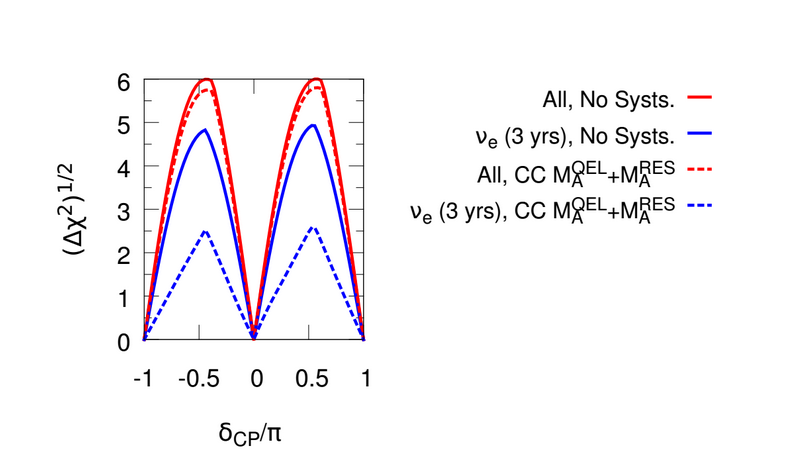
\includegraphics[width=0.8\linewidth]{figs/CPV_MARESQE.png}
% \caption{An example CP violation sensitivity calculated using inputs from the 
%   FastMC in a fit to all four ($\nu_e$, $\overline\nu_e$, $\nu_{\mu}$, 
%   $\overline\nu_{\mu}$) samples (red) and a fit to the $\nu_e$ appearance sample 
%   only (blue), for the case of no systematic uncertainty (solid) and the case in
%   which both $M_A^{QE,CC}$ and $M_A^{RES,CC}$ are allowed to vary with a
%   1$\sigma$ uncertainty of 20\% (dashed). This example was taken from an earlier
%   DUNE study, so the absolute sensitivity can not be compared with the DUNE 
%   sensitivities presented in this document.}
% \label{fig:MAresqesyst}
% \end{figure}

Uncertainty from nuclear interactions, in which particles exiting the primary
interaction vertex interact with the nuclear medium prior to depositing energy
in the detector, and detector effects, such as resolutions and energy scale
uncertainty, are somewhat more difficult to address with early simulation efforts.
However, in analogy to the treatment of cross-section uncertainty described above,
the effect of varying nuclear interaction parameters within their GENIE
uncertainties and comparisons of GENIE predictions to those of other
event generators are in progress.
Efforts to improve modeling of nuclear interactions and to develop 
reconstruction and analysis tools for a full Monte Carlo simulation are also underway. 
At the same time,
a number of test-beam and prototype experiments, including the DUNE 35-t prototype,
LARIAT, CAPTAIN, and the CERN neutrino platform experiments, are being designed and built to reduce these
uncertainties with experimental data.
